%%%%%%%%%%%%%%%%%%%%%%%%%%%%%%%%%%%%%%%%%%%%%%%%%%%%%%%%%%%%%%%%%%%%%%%%%%%%%%%%%
% Waterloo Rocketry Standard template for operations procedures                 %
% Copyright claimed by Aaron Morrison (akmorris@uwaterloo.ca)                   %
% Any commercial entity wishing to use this template in any way must provide    %
% to Waterloo Rocketry, one two-four (24 pack) of a non-shitty                  %
% type of beer or an amount of Canadian dollars roughly equalling               %
% the current cost of such a purchase. If you do so, then use it                %
% however you want, and I claim in no way that it compiles properly,            %
% and I take no responsibilty for any loss you incurr from using                %
% this template, and make no promises to support you in any technical           %
% capacity for sustained use.                                                   %
%%%%%%%%%%%%%%%%%%%%%%%%%%%%%%%%%%%%%%%%%%%%%%%%%%%%%%%%%%%%%%%%%%%%%%%%%%%%%%%%%
%%%%%%%%%%%%%%%%%%%%%%%%%%%%%%%%%%%%%%%%%%%%%%%%%%%%%%%%%%%%%%%%%%%%%%%%%%%%%%%%%
% Waterloo Rocketry Standard template for operations procedures                 %
% Copyright claimed by Aaron Morrison (akmorris@uwaterloo.ca)                   %
% Any commercial entity wishing to use this template in any way must provide    %
% to Waterloo Rocketry, one two-four (24 pack) of a non-shitty                  %
% type of beer or an amount of Canadian dollars roughly equalling               %
% the current cost of such a purchase. If you do so, then use it                %
% however you want, and I claim in no way that it compiles properly,            %
% and I take no responsibilty for any loss you incurr from using                %
% this template, and make no promises to support you in any technical           %
% capacity for sustained use.                                                   %
%%%%%%%%%%%%%%%%%%%%%%%%%%%%%%%%%%%%%%%%%%%%%%%%%%%%%%%%%%%%%%%%%%%%%%%%%%%%%%%%%
\documentclass[letter]{article}

%% margins and fonts
\usepackage[margin=1in]{geometry}
\renewcommand{\familydefault}{\sfdefault}

% begin package imports -- {{{
\usepackage{amsmath}
\usepackage{graphicx}
\usepackage[dvipsnames]{xcolor}
\usepackage{tabto}
\usepackage{titling}
\usepackage[iso,german]{isodate}
% end package imports -- }}}

% begin set section title styles -- {{{
\usepackage{titlesec}
\titleformat{\section} {\setcounter{checklistnum}{0} \normalfont\Large\bfseries}{}{0em}{}[{\titlerule[0.8pt]}]
\titleformat{\subsection} {\setcounter{checklistnum}{0} \normalfont\large}{}{0em}{}[{\titlerule[0.6pt]}]
% end set section title styles -- }}}

% begin checklist symbols definition -- {{{
\usepackage{enumitem,amssymb}
\newcounter{checklistnum}
\setcounter{checklistnum}{0}
\DeclareRobustCommand{\checklistnumber}{\refstepcounter{checklistnum}\thechecklistnum}
\newlist{checklist}{itemize}{6}
\setlist[checklist,1]{
label={\color{gray}\checklistnumber}\hspace{2em}$\square$,
leftmargin=0em,
itemindent=2em
}
\setlist[checklist,2]{
label={\color{gray}\checklistnumber}\hspace{4em}$\square$,
leftmargin=0em,
itemindent=4em
}
\setlist[checklist,3]{
label={\color{gray}\checklistnumber}\hspace{6em}$\square$,
leftmargin=0em,
itemindent=6em
}
\setlist[checklist,4]{
label={\color{gray}\checklistnumber}\hspace{8em}$\square$,
leftmargin=0em,
itemindent=8em
}
\setlist[checklist,5]{
label={\color{gray}\checklistnumber}\hspace{10em}$\square$,
leftmargin=0em,
itemindent=10em
}
\setlist[checklist,6]{
label={\color{gray}\checklistnumber}\hspace{12em}$\square$,
leftmargin=0em,
itemindent=12em
}
% end checklist symbols definition -- }}}

% begin personnel macro -- {{{
\newcommand{\operator}[4]{%
  \expandafter\newcommand\csname #1\endcsname{{\color{#2}\textbf{#3}}\phantom{}}
  \expandafter\newcommand\csname #1full\endcsname{{\color{#2}\textbf{#4 [#3]}}\phantom{}}
}
% end personnel macro -- }}}

\pagenumbering{gobble}

\usepackage{pdfpages}

\title{
\Huge Canadian Reduced Gravity Experiment 2019: Project Maple\\
\vspace{1cm}
\Large CAN-RGX Experiment Assembly and Operations Procedures}


\begin{document}

% begin titlepage -- {{{
\begin{center}
\vspace*{7cm}
\hspace{7em}
\includegraphics[width=30em]{common/mono_horizontal_standard}
\newline
\rule{50em}{2pt}

\vspace{1cm}
\thetitle

\vspace*{\fill}
Compiled on \today
\end{center}
\newpage
% end titlepage -- }}}


\section{Background and Reference}

% begin operators declarations -- {{{
% syntax for operator macro:
% arg1: their name (so here you use \auth to insert the AUTHOR name)
% arg2: the color you want them highlighted in
% arg3: their abbreviated title (what you should use in the checklists)
% arg4: their full title (insert into document with arg1 + full, so for auth
%       it'd be "\authfull" to insert their full title). Use this in Personnel
%       Required subsection, and in Sign Off subsection.
\operator{commander}{red}{Payload Commander}{Riley}
\operator{payload}{Green}{Payload Specialist}{Kyle}
\operator{mspecpri}{blue}{Mission Specialist 1}{Teresa}
\operator{mspecsec}{blue}{Mission Specialist 2}{Aaron}
% end operators declarations -- }}}

% begin contents subsection -- {{{
\subsection{Contents}
This document contains the following:
\begin{itemize}
    \item \textbf{N1} \textit{Experiment Assembly} comprised of all steps that can be completed before the day of flight.
    \item \textbf{N2} \textit{Pre-Flight Setup} comprised of all steps to be completed immediately before boarding the Falcon.
    \item \textbf{N3} \textit{In-Flight Operations} comprised of setup, experiment procedures, and contingency plans to be executed aboard the Falcon.
\end{itemize}
% end contents subsection -- }}}

% begin personnel required section -- {{{
\subsection{Personnel Required}
There are 4 people required for us performing at CAN-RGX.
\begin{checklist}
    \item \commanderfull{} is responsible for organizing and overseeing operations and crew, as well as liaising with SEDS and NRC staff. Primary operator for setup and experiment procedures.
    \item \payloadfull{} is responsible for assisting the \commander{} with experiment setup and operation. Both the \payload{} and the \commander{} will be flying in reduced gravity aboard the Falcon.
    \item \mspecprifull{} and \mspecsecfull{} are responsible for assisting the flight operators with ground based setup and debugging on the tarmac before \commander{} and \payload{} board the Falcon. In event of either flight operators being unable to participate in flight, either \mspecpri{} or \mspecsec{} will take their place and responsibilties onboard the Falcon.
\end{checklist}
\setcounter{checklistnum}{0}
% end personnel required section -- }}}

% begin sign off -- {{{
\subsection{Sign-Off}
\textit{To be completed by all CAN-RGX personnel after reading and familiarization with procedures}
\begin{checklist}
    \item \commanderfull      \tabto{25em}\rule{10em}{0.4pt}\hspace{5em}\rule{10em}{0.4pt}
    \item \payloadfull        \tabto{25em}\rule{10em}{0.4pt}\hspace{5em}\rule{10em}{0.4pt}
    \item \mspecprifull       \tabto{25em}\rule{10em}{0.4pt}\hspace{5em}\rule{10em}{0.4pt}
    \item \mspecsecfull       \tabto{25em}\rule{10em}{0.4pt}\hspace{5em}\rule{10em}{0.4pt}
\end{checklist}
\setcounter{checklistnum}{0}
% end sign off -- }}}

% begin assembly checklist-- {{{
\newpage
\section{[N1] Experiment Assembly}
\begin{checklist}
    \item Ensure Velcro straps over cell boxes make a secure connection and are not prone to accidental removal.
    \item Lay out a sheet of shop towel, and place all test cells vertically on top of this sheet.
    \item One at a time, fill the test cells with coloured water using a syringe and pipette. Filled cells will be searched for immediate leaks.
    \begin{checklist}
        \item If a cell leaks immediately, it should be quickly drained, marked as leaky and set aside. This cell will be excluded from the experiment.
        \item Cells that do not show any immediate signs of leaks will be plugged:
        \begin{checklist}
            \item Using Q-tip, apply a thin coating of Vaseline to a shortened rubber stopper.
            \item The lubricated stopper will be pushed and subsequently twisted into the
fill port of the cell in question.
            \item A light bead of hot glue will be applied around the base of the stopper.
        \end{checklist}
        \item Plugged cells will be placed face down on the shop towel and left for at least 30 minutes, longer if schedule allows.  Procedure shall continue while cells are sitting.
    \end{checklist}
    \item Using 3/16'' and 4mm Allen keys for 1/4-20 and M5 screws (respectively), check tightness of all fasteners.
    \item Check connection of lights on lid, ensure they aren’t prone to falling off.
    \item Connect camera remote to cell phone, and plug phone charger into Pelican Case.
    \item Secure camera into phone holder, and plug into charger.
    \begin{checklist}
        \item Ensure phone is charging properly.
        \item Use remote to start video on the camera.
        \item Close case lid and use light remote to turn on interior lights to 40\% brightness.
        \item Wait several seconds, then turn off camera and lights and open the Pelican Case.
    \end{checklist}
    \item Open storage information of phone camera.
    \begin{checklist}
        \item If $>$10 GB is available, phone setup is complete.
        \item If 10 GB of storage is not free, go to files, photos and videos and delete enough to ensure $>$10 GB of storage is free.
        \item Repeat step 9 with backup camera.
    \end{checklist}
    \item Once all setup is complete and half-hour has been waited, check fluid cells again for leaks apparent on the shop towel.
    \begin{checklist}
        \item Any cells with leaks shall be drained, and set aside for exclusion from the experiment.
        \item Cells that are not leaking shall be drained, and replaced in their holding boxes. Draining will be performed as follows:
        \begin{checklist}
            \item The ring of glue will be pulled off using a dental pick.
            \item Rubber stopper will be carefully removed using side-to-side motion.
            \item Vaseline will be cleaned off of rubber stopper with shop tower.
            \item Cell will be inverted over a waste container and gently patted until all fluid is drained.
        \end{checklist}
    \end{checklist}
    \item Ensure test cells fit well in cell sites, and the Velcro adhering them holds firm.
\end{checklist}
\textbf{End of Experiment Assembly}
% end assembly -- }}}

% beginnning of pre-flight setup checklist -- {{{
\newpage{}
\section{[N2] Pre-Flight Setup}
\begin{checklist}
	\item One at a time, the remaining valid test cells are to be filled with their designated amounts of ferrofluid using a syringe and pipette.
    \begin{checklist}
        \item Each geometry of cell will have the first cell filled to 1/3 fill height, the second to 1/2 fill height.
        \item Filling will consist of the following:
        \begin{checklist}
			\item Shoot 3-6 mL of WD-40 in the test cell.
			\item Shake and move cell around to coat walls in WD-40.
			\item Use first syringe, then pipette to carefully transfer ferrofluid from its bottle into the test cell.
        \end{checklist}
    \end{checklist}
	\item After each fill, the test cell in question will be plugged:
    \begin{checklist}
		\item A shortened rubber stopper will be lightly greased with Vaseline, using a Q-tip.
		\item The greased stopper will be pushed and then twisted into the fill port of the cell in question.
		\item A thin bead of hot glue will be applied around the base of the stopper.
    \end{checklist}
	\item Each cell will be examined closely for any fluid leaks. Any leaking cells will be emptied and removed from the experiment.
	\item Any changes necessary to cell numbering due to excluded test cells will be made now at the discretion of the Mission Specialists.
	\item When all cells are filled, they are to be loaded into their holding boxes and secured with the Velcro strap.
	\item The camera phone will be secured in its holder and plugged into the pelican case for charging.
	\item Connectivity between light, phone and their respective remotes will be ensured before they are turned off and the Pelican Case is closed.
	\item Experiment is now ready for integration with the Falcon 20, pending recommendations by NRC staff.
\end{checklist}
\textbf{End of Pre-Flight Setup}
% end of pre-flight -- }}}

% beginnning of in-flight checklist -- {{{
\newpage{}
\section{In-Flight Operations}
% beginning of level flight setup -- {{{
\subsection{Level Flight Setup}
The following will be performed during every level flight section between
parabolas.  A detailed list of which cells and magnet positions
are to be used for each parabola can be found immediately following this
section.
\begin{checklist}
    \item If anything is noticed to be broken, loose, or otherwise in need of repair, the parts in question will be fixed at the discretion of the operating technicians.
    \item Any unnecessary test cells in test sites will be removed by pulling on their securing Velcro.  Remove the new test cells from their holding boxes and attach them to the test sites using the Velcro.  The cell boxes will be resecured with their Velcro straps.
    \item Required magnets will be removed from their holding cases in the toolbox and placed into the specified test holder locations. Any magnets previously installed that are not necessary will be removed.  Needle-nosed pliers (found in toolbox) may be needed to remove magnets.
    \item All tools used will be returned to their designated storage place, all loose parts will be secured and the lid of the Pelican Case will be closed.
\end{checklist}
\textbf{The following steps need only be performed on the first setup period and will be left on for the remainder of the flight.}
\begin{checklist}
    \item Once lid is closed, camera will be turned on by remote.
    \item Interior lights will be turned on to 40\% brightness by remote.
\end{checklist}
% beginning of level flight setup -- }}}

% beginning of experiment parabola table -- {{{
\definecolor{yellow3}{RGB}{255,213,79}
\definecolor{tablegrey}{RGB}{230,230,230}
{ \Large
\begin{center}
    \begin{tabular} {|l|l|c|}
        \rowcolor{yellow3} \hline
            Parabola \# & Test cells in use & Magnet Positions \\
        \hline
            1 & 1,2,3,4 & O    \\
        \rowcolor{tablegrey} \hline
            2 & 5,6,7,8 & O    \\
        \hline
            3 & 9,10,11,12 & O    \\
        \rowcolor{tablegrey} \hline
            4 & 9,10,11,12 & L    \\
        \hline
            5 & 1,2,3,4 & L    \\
        \rowcolor{tablegrey} \hline
            6 & 5,6,7,8 & L    \\
        \hline
            7 & 5,6,7,8 & L, R \\
        \rowcolor{tablegrey} \hline
            8 & 9,10,11,12 & L, R \\
        \hline
            9 & 1,2,3,4 & L, R \\
        \rowcolor{tablegrey} \hline
            10& 1,2,3,4 & L, R \\
        \hline
    \end{tabular}
\end{center}
}
% end of experiment parabola table -- }}}

% beginning of emergency operations -- {{{
\newpage
\subsection{Reduced Gravity and Emergency Operations}
The following will be performed for every reduced gravity section of flight.
Exact details about the current configuration can be found in the table above.

\begin{checklist}

	\item The experiment will be left to run on its own, as it is fully passive. During operation, Mission Specialists are to be watching for anything that goes wrong or needs attention. This section is intended for use in case of mishaps.
	\item Ferrofluid Spill/leak:
    \begin{checklist}
		\item The leaking cell will be identified, removed from the test site and wrapped in absorbent cloth.
		\item Cell and cloth will be placed in a large Ziploc bag, the bag will be sealed and placed in the flight toolbox.
		\item If fluid has contaminated any parts of the experiment, it will be cleaned up with absorbent cloth and water (if necessary).
		\item Leaking cell will be excluded from operations and the experiment may continue, provided there is no extensive damage to the system.
    \end{checklist}
	\item Power Loss:
    \begin{checklist}
        \item Experiment will continue without charging to phone camera.
    \end{checklist}
	\item Camera Failure:
    \begin{checklist}
		\item Should the camera stop recording, or be incapacitated in some other way, it will be promptly removed from the experiment.
		\item The secondary Mission Specialist will have a phone camera on their person that will be substituted for the original.
		\item The experiment can proceed using new hardware.
    \end{checklist}
	\item Motion sick/unconscious crew member:
    \begin{checklist}
		\item For minor motion sickness, crew will follow given minimization tactics and wait for sickness to pass.
		\item For severe cases and unconsciousness, NRC staff will be alerted and judgement will be deferred to qualified staff.
    \end{checklist}
\end{checklist}
% end of emergency operations -- }}}
\textbf{End of In-Flight Operations}
% end of in-flight -- }}}

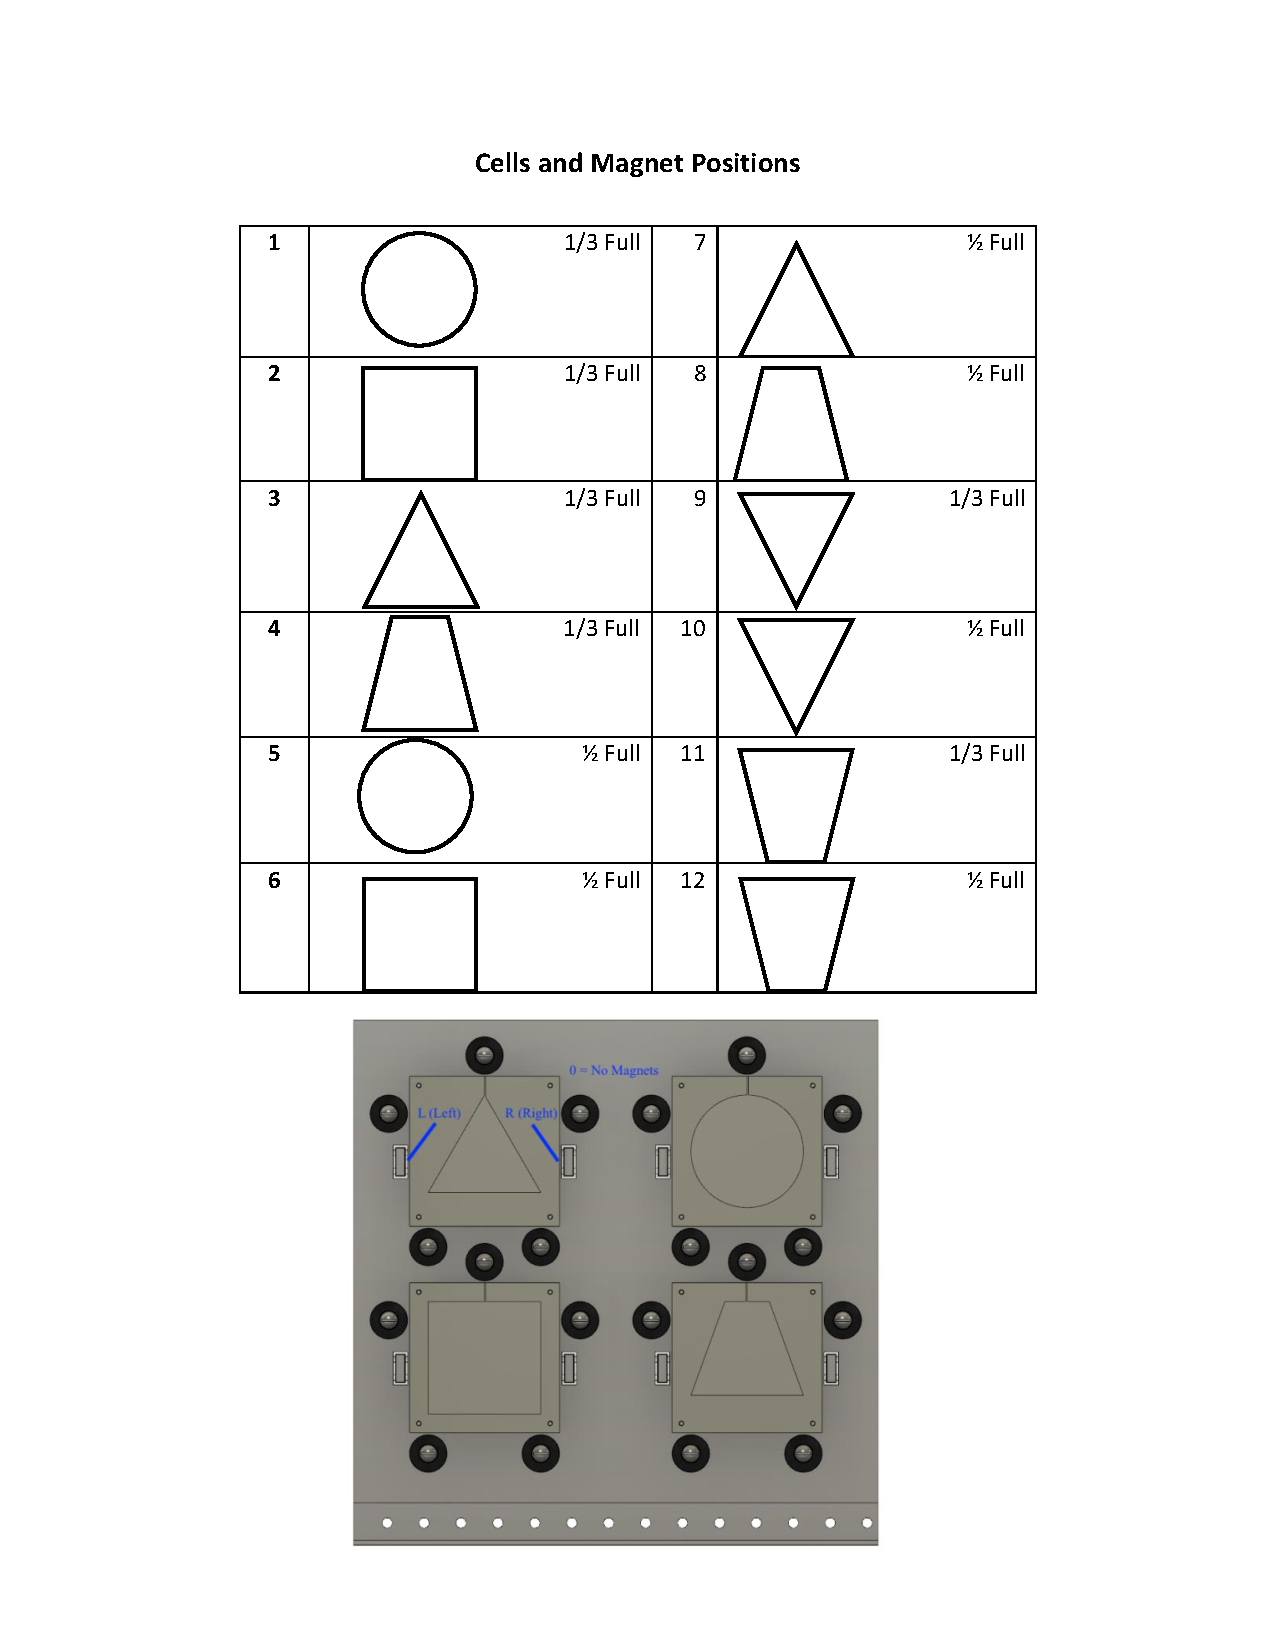
\includepdf[pages=-]{images/can_rgx_2019_cell_magnet_table.pdf}

\end{document}
